\documentclass[]{article}
\usepackage{lmodern}
\usepackage{amssymb,amsmath}
\usepackage{ifxetex,ifluatex}
\usepackage{fixltx2e} % provides \textsubscript
\ifnum 0\ifxetex 1\fi\ifluatex 1\fi=0 % if pdftex
  \usepackage[T1]{fontenc}
  \usepackage[utf8]{inputenc}
\else % if luatex or xelatex
  \ifxetex
    \usepackage{mathspec}
  \else
    \usepackage{fontspec}
  \fi
  \defaultfontfeatures{Ligatures=TeX,Scale=MatchLowercase}
\fi
% use upquote if available, for straight quotes in verbatim environments
\IfFileExists{upquote.sty}{\usepackage{upquote}}{}
% use microtype if available
\IfFileExists{microtype.sty}{%
\usepackage{microtype}
\UseMicrotypeSet[protrusion]{basicmath} % disable protrusion for tt fonts
}{}
\usepackage[margin=1in]{geometry}
\usepackage{hyperref}
\hypersetup{unicode=true,
            pdftitle={Plotting},
            pdfauthor={Jennifer Brazeal},
            pdfborder={0 0 0},
            breaklinks=true}
\urlstyle{same}  % don't use monospace font for urls
\usepackage{color}
\usepackage{fancyvrb}
\newcommand{\VerbBar}{|}
\newcommand{\VERB}{\Verb[commandchars=\\\{\}]}
\DefineVerbatimEnvironment{Highlighting}{Verbatim}{commandchars=\\\{\}}
% Add ',fontsize=\small' for more characters per line
\usepackage{framed}
\definecolor{shadecolor}{RGB}{248,248,248}
\newenvironment{Shaded}{\begin{snugshade}}{\end{snugshade}}
\newcommand{\AlertTok}[1]{\textcolor[rgb]{0.94,0.16,0.16}{#1}}
\newcommand{\AnnotationTok}[1]{\textcolor[rgb]{0.56,0.35,0.01}{\textbf{\textit{#1}}}}
\newcommand{\AttributeTok}[1]{\textcolor[rgb]{0.77,0.63,0.00}{#1}}
\newcommand{\BaseNTok}[1]{\textcolor[rgb]{0.00,0.00,0.81}{#1}}
\newcommand{\BuiltInTok}[1]{#1}
\newcommand{\CharTok}[1]{\textcolor[rgb]{0.31,0.60,0.02}{#1}}
\newcommand{\CommentTok}[1]{\textcolor[rgb]{0.56,0.35,0.01}{\textit{#1}}}
\newcommand{\CommentVarTok}[1]{\textcolor[rgb]{0.56,0.35,0.01}{\textbf{\textit{#1}}}}
\newcommand{\ConstantTok}[1]{\textcolor[rgb]{0.00,0.00,0.00}{#1}}
\newcommand{\ControlFlowTok}[1]{\textcolor[rgb]{0.13,0.29,0.53}{\textbf{#1}}}
\newcommand{\DataTypeTok}[1]{\textcolor[rgb]{0.13,0.29,0.53}{#1}}
\newcommand{\DecValTok}[1]{\textcolor[rgb]{0.00,0.00,0.81}{#1}}
\newcommand{\DocumentationTok}[1]{\textcolor[rgb]{0.56,0.35,0.01}{\textbf{\textit{#1}}}}
\newcommand{\ErrorTok}[1]{\textcolor[rgb]{0.64,0.00,0.00}{\textbf{#1}}}
\newcommand{\ExtensionTok}[1]{#1}
\newcommand{\FloatTok}[1]{\textcolor[rgb]{0.00,0.00,0.81}{#1}}
\newcommand{\FunctionTok}[1]{\textcolor[rgb]{0.00,0.00,0.00}{#1}}
\newcommand{\ImportTok}[1]{#1}
\newcommand{\InformationTok}[1]{\textcolor[rgb]{0.56,0.35,0.01}{\textbf{\textit{#1}}}}
\newcommand{\KeywordTok}[1]{\textcolor[rgb]{0.13,0.29,0.53}{\textbf{#1}}}
\newcommand{\NormalTok}[1]{#1}
\newcommand{\OperatorTok}[1]{\textcolor[rgb]{0.81,0.36,0.00}{\textbf{#1}}}
\newcommand{\OtherTok}[1]{\textcolor[rgb]{0.56,0.35,0.01}{#1}}
\newcommand{\PreprocessorTok}[1]{\textcolor[rgb]{0.56,0.35,0.01}{\textit{#1}}}
\newcommand{\RegionMarkerTok}[1]{#1}
\newcommand{\SpecialCharTok}[1]{\textcolor[rgb]{0.00,0.00,0.00}{#1}}
\newcommand{\SpecialStringTok}[1]{\textcolor[rgb]{0.31,0.60,0.02}{#1}}
\newcommand{\StringTok}[1]{\textcolor[rgb]{0.31,0.60,0.02}{#1}}
\newcommand{\VariableTok}[1]{\textcolor[rgb]{0.00,0.00,0.00}{#1}}
\newcommand{\VerbatimStringTok}[1]{\textcolor[rgb]{0.31,0.60,0.02}{#1}}
\newcommand{\WarningTok}[1]{\textcolor[rgb]{0.56,0.35,0.01}{\textbf{\textit{#1}}}}
\usepackage{graphicx,grffile}
\makeatletter
\def\maxwidth{\ifdim\Gin@nat@width>\linewidth\linewidth\else\Gin@nat@width\fi}
\def\maxheight{\ifdim\Gin@nat@height>\textheight\textheight\else\Gin@nat@height\fi}
\makeatother
% Scale images if necessary, so that they will not overflow the page
% margins by default, and it is still possible to overwrite the defaults
% using explicit options in \includegraphics[width, height, ...]{}
\setkeys{Gin}{width=\maxwidth,height=\maxheight,keepaspectratio}
\IfFileExists{parskip.sty}{%
\usepackage{parskip}
}{% else
\setlength{\parindent}{0pt}
\setlength{\parskip}{6pt plus 2pt minus 1pt}
}
\setlength{\emergencystretch}{3em}  % prevent overfull lines
\providecommand{\tightlist}{%
  \setlength{\itemsep}{0pt}\setlength{\parskip}{0pt}}
\setcounter{secnumdepth}{0}
% Redefines (sub)paragraphs to behave more like sections
\ifx\paragraph\undefined\else
\let\oldparagraph\paragraph
\renewcommand{\paragraph}[1]{\oldparagraph{#1}\mbox{}}
\fi
\ifx\subparagraph\undefined\else
\let\oldsubparagraph\subparagraph
\renewcommand{\subparagraph}[1]{\oldsubparagraph{#1}\mbox{}}
\fi

%%% Use protect on footnotes to avoid problems with footnotes in titles
\let\rmarkdownfootnote\footnote%
\def\footnote{\protect\rmarkdownfootnote}

%%% Change title format to be more compact
\usepackage{titling}

% Create subtitle command for use in maketitle
\providecommand{\subtitle}[1]{
  \posttitle{
    \begin{center}\large#1\end{center}
    }
}

\setlength{\droptitle}{-2em}

  \title{Plotting}
    \pretitle{\vspace{\droptitle}\centering\huge}
  \posttitle{\par}
    \author{Jennifer Brazeal}
    \preauthor{\centering\large\emph}
  \postauthor{\par}
      \predate{\centering\large\emph}
  \postdate{\par}
    \date{9/5/19}


\begin{document}
\maketitle

Save data from internal \texttt{datasets} package as a new object. This
dataset is observations of CO2 uptake by plants originating from
different locations, and with different temperature treatments
performed.

\begin{Shaded}
\begin{Highlighting}[]
\NormalTok{CO2 =}\StringTok{ }\NormalTok{datasets}\OperatorTok{::}\NormalTok{CO2}
\end{Highlighting}
\end{Shaded}

Remind us what it looks like - three columns of character vectors
represented as `factors', and two numeric columns

\begin{Shaded}
\begin{Highlighting}[]
\KeywordTok{head}\NormalTok{(CO2)}
\end{Highlighting}
\end{Shaded}

\begin{verbatim}
##   Plant   Type  Treatment conc uptake
## 1   Qn1 Quebec nonchilled   95   16.0
## 2   Qn1 Quebec nonchilled  175   30.4
## 3   Qn1 Quebec nonchilled  250   34.8
## 4   Qn1 Quebec nonchilled  350   37.2
## 5   Qn1 Quebec nonchilled  500   35.3
## 6   Qn1 Quebec nonchilled  675   39.2
\end{verbatim}

More specific information about the structure (str) of the data

\begin{Shaded}
\begin{Highlighting}[]
\KeywordTok{str}\NormalTok{(CO2)}
\end{Highlighting}
\end{Shaded}

\begin{verbatim}
## Classes 'nfnGroupedData', 'nfGroupedData', 'groupedData' and 'data.frame':   84 obs. of  5 variables:
##  $ Plant    : Ord.factor w/ 12 levels "Qn1"<"Qn2"<"Qn3"<..: 1 1 1 1 1 1 1 2 2 2 ...
##  $ Type     : Factor w/ 2 levels "Quebec","Mississippi": 1 1 1 1 1 1 1 1 1 1 ...
##  $ Treatment: Factor w/ 2 levels "nonchilled","chilled": 1 1 1 1 1 1 1 1 1 1 ...
##  $ conc     : num  95 175 250 350 500 675 1000 95 175 250 ...
##  $ uptake   : num  16 30.4 34.8 37.2 35.3 39.2 39.7 13.6 27.3 37.1 ...
##  - attr(*, "formula")=Class 'formula'  language uptake ~ conc | Plant
##   .. ..- attr(*, ".Environment")=<environment: R_EmptyEnv> 
##  - attr(*, "outer")=Class 'formula'  language ~Treatment * Type
##   .. ..- attr(*, ".Environment")=<environment: R_EmptyEnv> 
##  - attr(*, "labels")=List of 2
##   ..$ x: chr "Ambient carbon dioxide concentration"
##   ..$ y: chr "CO2 uptake rate"
##  - attr(*, "units")=List of 2
##   ..$ x: chr "(uL/L)"
##   ..$ y: chr "(umol/m^2 s)"
\end{verbatim}

\hypertarget{visualization-types}{%
\section{Visualization types}\label{visualization-types}}

\hypertarget{plots-of-data-distribution-in-one-dimension}{%
\subsection{Plots of data distribution in one
dimension}\label{plots-of-data-distribution-in-one-dimension}}

\hypertarget{histogram---group-the-data-into-bins-default-or-custom-defined-spanning-the-range-of-the-data-and-display-frequency-of-each-bin.}{%
\subsubsection{Histogram - group the data into bins (default or custom
defined) spanning the range of the data and display frequency of each
bin.}\label{histogram---group-the-data-into-bins-default-or-custom-defined-spanning-the-range-of-the-data-and-display-frequency-of-each-bin.}}

\begin{Shaded}
\begin{Highlighting}[]
\NormalTok{?hist}
\end{Highlighting}
\end{Shaded}

\begin{verbatim}
## starting httpd help server ... done
\end{verbatim}

Example:

\begin{Shaded}
\begin{Highlighting}[]
\KeywordTok{hist}\NormalTok{(CO2}\OperatorTok{$}\NormalTok{uptake)}
\end{Highlighting}
\end{Shaded}

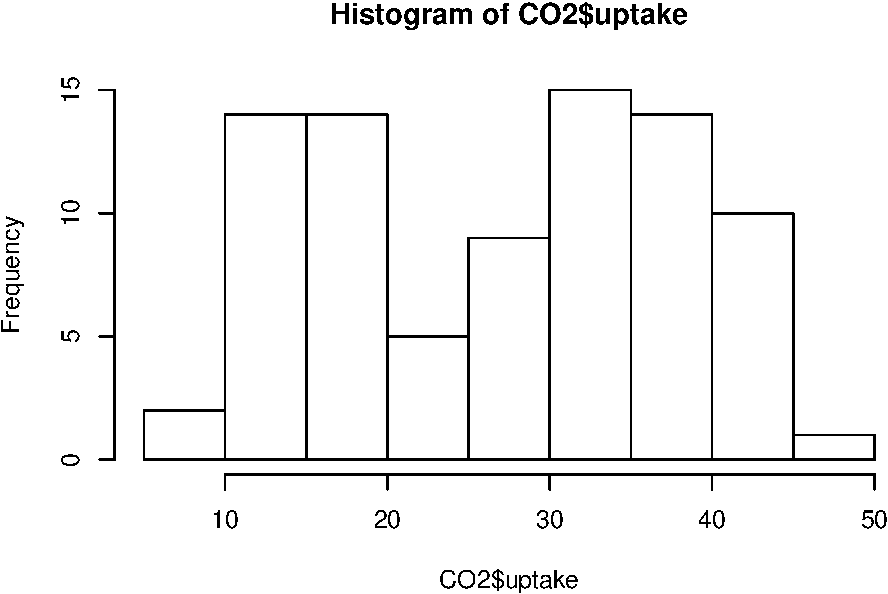
\includegraphics{Plotting_JB_files/figure-latex/unnamed-chunk-5-1.pdf}
\#\#\# Density - Smooth out the data and display density (analogous to
continuous frequency) of data along the range of the data.

\begin{Shaded}
\begin{Highlighting}[]
\NormalTok{?density }\CommentTok{# Combine with plot() to vizualize; i.e. plot(density(x))}
\end{Highlighting}
\end{Shaded}

Example:

\begin{Shaded}
\begin{Highlighting}[]
\KeywordTok{density}\NormalTok{(CO2}\OperatorTok{$}\NormalTok{uptake)}
\end{Highlighting}
\end{Shaded}

\begin{verbatim}
## 
## Call:
##  density.default(x = CO2$uptake)
## 
## Data: CO2$uptake (84 obs.);  Bandwidth 'bw' = 4.012
## 
##        x                y            
##  Min.   :-4.337   Min.   :2.286e-05  
##  1st Qu.:11.132   1st Qu.:2.863e-03  
##  Median :26.600   Median :2.125e-02  
##  Mean   :26.600   Mean   :1.615e-02  
##  3rd Qu.:42.068   3rd Qu.:2.649e-02  
##  Max.   :57.537   Max.   :3.095e-02
\end{verbatim}

\begin{Shaded}
\begin{Highlighting}[]
\KeywordTok{plot}\NormalTok{(}\KeywordTok{density}\NormalTok{(CO2}\OperatorTok{$}\NormalTok{uptake))}
\end{Highlighting}
\end{Shaded}

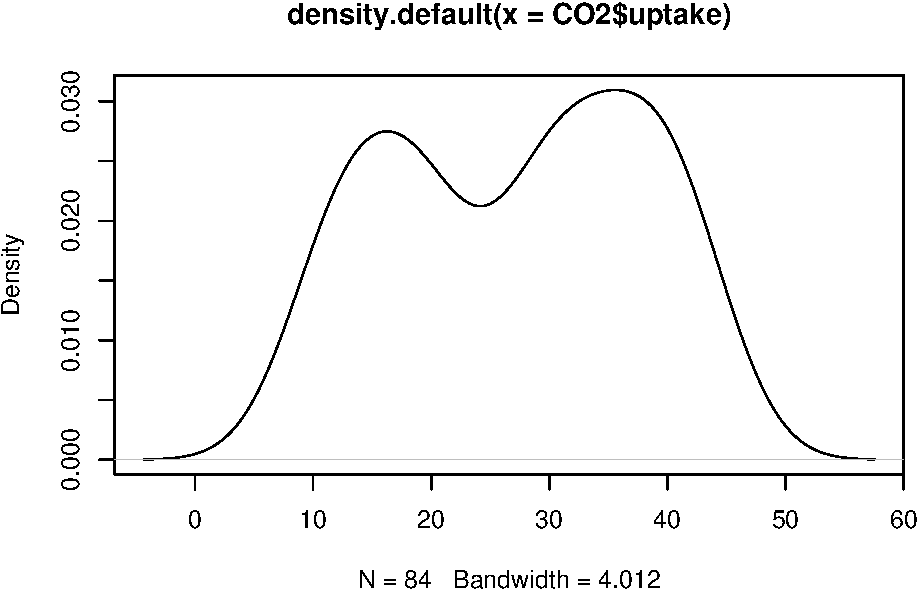
\includegraphics{Plotting_JB_files/figure-latex/unnamed-chunk-7-1.pdf}
\#\#\# Dotchart - Display all point values along one dimension.

\begin{Shaded}
\begin{Highlighting}[]
\NormalTok{?dotchart}
\end{Highlighting}
\end{Shaded}

Examples:\\
Note, you can specify a grouping factor (remember ``factor''?) to divide
the points and visually compare

\begin{Shaded}
\begin{Highlighting}[]
\KeywordTok{dotchart}\NormalTok{(CO2}\OperatorTok{$}\NormalTok{uptake)}
\end{Highlighting}
\end{Shaded}

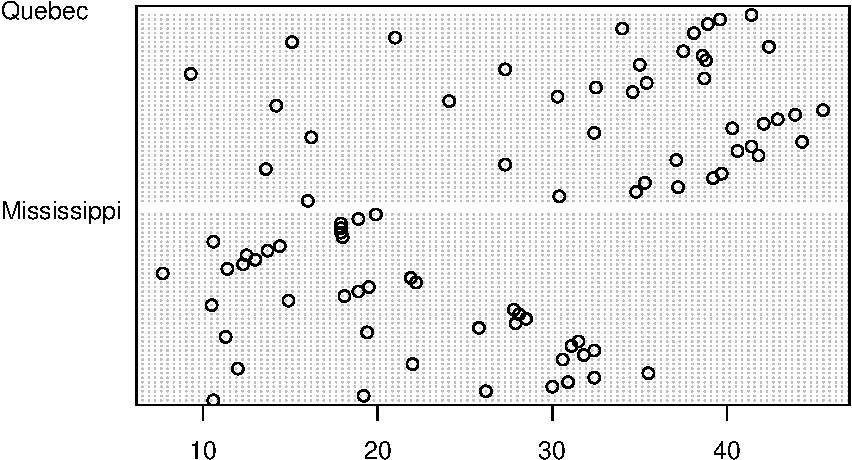
\includegraphics{Plotting_JB_files/figure-latex/unnamed-chunk-9-1.pdf}

\begin{Shaded}
\begin{Highlighting}[]
\KeywordTok{dotchart}\NormalTok{(CO2}\OperatorTok{$}\NormalTok{uptake, }\DataTypeTok{groups =}\NormalTok{ CO2}\OperatorTok{$}\NormalTok{Type)}
\end{Highlighting}
\end{Shaded}

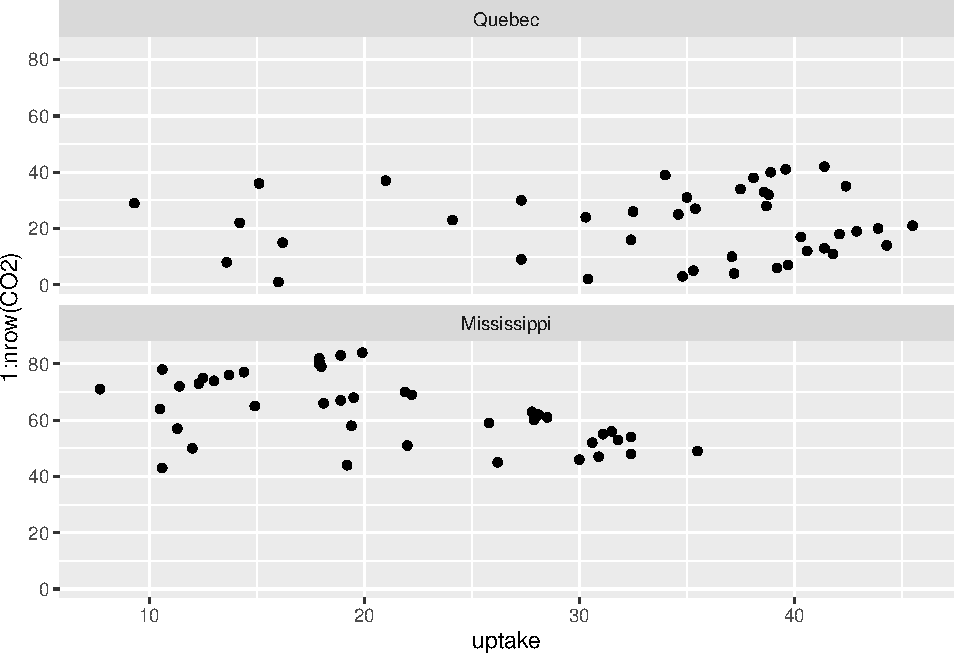
\includegraphics{Plotting_JB_files/figure-latex/unnamed-chunk-9-2.pdf}

\begin{Shaded}
\begin{Highlighting}[]
\KeywordTok{dotchart}\NormalTok{(CO2}\OperatorTok{$}\NormalTok{uptake, }\DataTypeTok{color =}\NormalTok{ CO2}\OperatorTok{$}\NormalTok{Type)}
\end{Highlighting}
\end{Shaded}

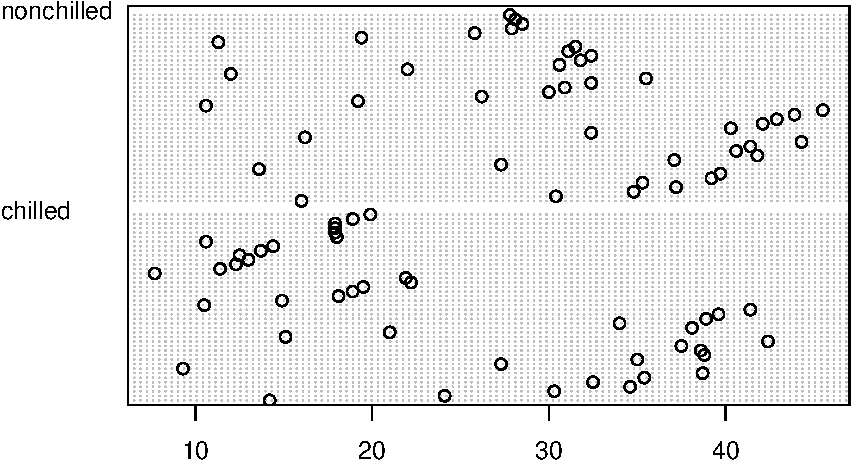
\includegraphics{Plotting_JB_files/figure-latex/unnamed-chunk-9-3.pdf}

\begin{Shaded}
\begin{Highlighting}[]
\KeywordTok{dotchart}\NormalTok{(CO2}\OperatorTok{$}\NormalTok{uptake, }\DataTypeTok{groups =}\NormalTok{ CO2}\OperatorTok{$}\NormalTok{Treatment)}
\end{Highlighting}
\end{Shaded}

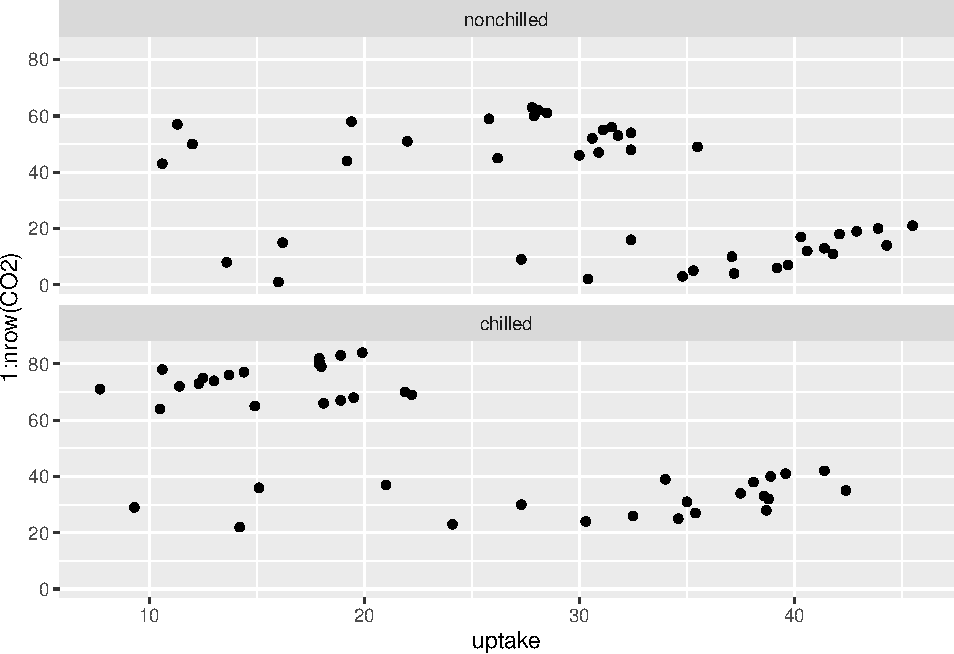
\includegraphics{Plotting_JB_files/figure-latex/unnamed-chunk-9-4.pdf}

\begin{Shaded}
\begin{Highlighting}[]
\KeywordTok{dotchart}\NormalTok{(CO2}\OperatorTok{$}\NormalTok{uptake, }\DataTypeTok{color =}\NormalTok{ CO2}\OperatorTok{$}\NormalTok{Treatment)}
\end{Highlighting}
\end{Shaded}

\includegraphics{Plotting_JB_files/figure-latex/unnamed-chunk-9-5.pdf}

\hypertarget{plots-in-two-dimension}{%
\subsection{Plots in two-dimension}\label{plots-in-two-dimension}}

\hypertarget{ordinary-point-plotting}{%
\subsubsection{Ordinary point plotting}\label{ordinary-point-plotting}}

\hypertarget{there-are-many-arguments-which-allow-you-to-alter-the-look-of-your-plot}{%
\subsection{There are many arguments which allow you to alter the look
of your
plot:}\label{there-are-many-arguments-which-allow-you-to-alter-the-look-of-your-plot}}

\begin{Shaded}
\begin{Highlighting}[]
\NormalTok{?plot }\CommentTok{# Plot points along x and y axes. Follow with points() for additional points from related data, or lines(); examples below.}
\end{Highlighting}
\end{Shaded}

Examples:

\begin{Shaded}
\begin{Highlighting}[]
\CommentTok{# We will introduce a different dataset no}
\NormalTok{iris <-}\StringTok{ }\NormalTok{datasets}\OperatorTok{::}\NormalTok{iris}
\KeywordTok{head}\NormalTok{(iris)}
\end{Highlighting}
\end{Shaded}

\begin{verbatim}
##   Sepal.Length Sepal.Width Petal.Length Petal.Width Species
## 1          5.1         3.5          1.4         0.2  setosa
## 2          4.9         3.0          1.4         0.2  setosa
## 3          4.7         3.2          1.3         0.2  setosa
## 4          4.6         3.1          1.5         0.2  setosa
## 5          5.0         3.6          1.4         0.2  setosa
## 6          5.4         3.9          1.7         0.4  setosa
\end{verbatim}

\begin{Shaded}
\begin{Highlighting}[]
\NormalTok{?iris}
\end{Highlighting}
\end{Shaded}

We can use a scatterplot to look at how petal length changes with sepal
length:

\begin{Shaded}
\begin{Highlighting}[]
\KeywordTok{plot}\NormalTok{(iris}\OperatorTok{$}\NormalTok{Sepal.Length, iris}\OperatorTok{$}\NormalTok{Petal.Length)}
\end{Highlighting}
\end{Shaded}

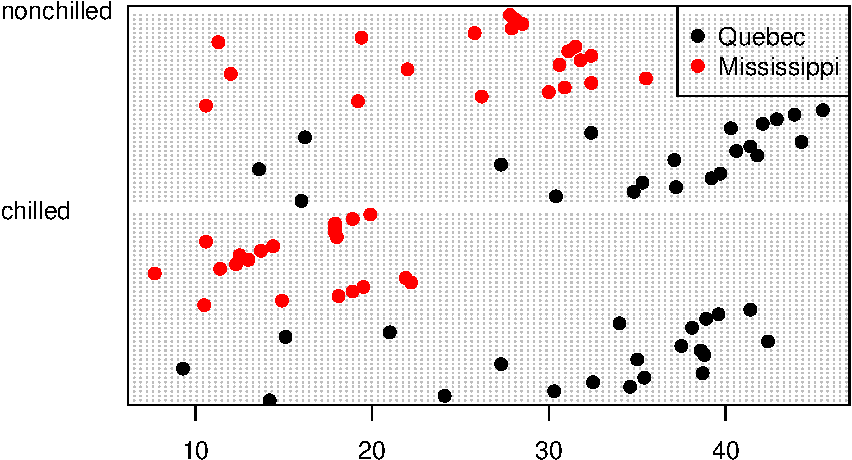
\includegraphics{Plotting_JB_files/figure-latex/unnamed-chunk-12-1.pdf}

\hypertarget{box-plot---group-the-data-along-discrete-factors-and-display-median-interquartile-range-whiskers-and-outliers}{%
\subsection{Box plot - Group the data along discrete factors, and
display median, interquartile range (whiskers), and
outliers}\label{box-plot---group-the-data-along-discrete-factors-and-display-median-interquartile-range-whiskers-and-outliers}}

You can also specify a categorical (factor level) x variable, which will
automatically produce a boxplot:

\begin{Shaded}
\begin{Highlighting}[]
\KeywordTok{plot}\NormalTok{(iris}\OperatorTok{$}\NormalTok{Species, iris}\OperatorTok{$}\NormalTok{Petal.Length) }
\end{Highlighting}
\end{Shaded}

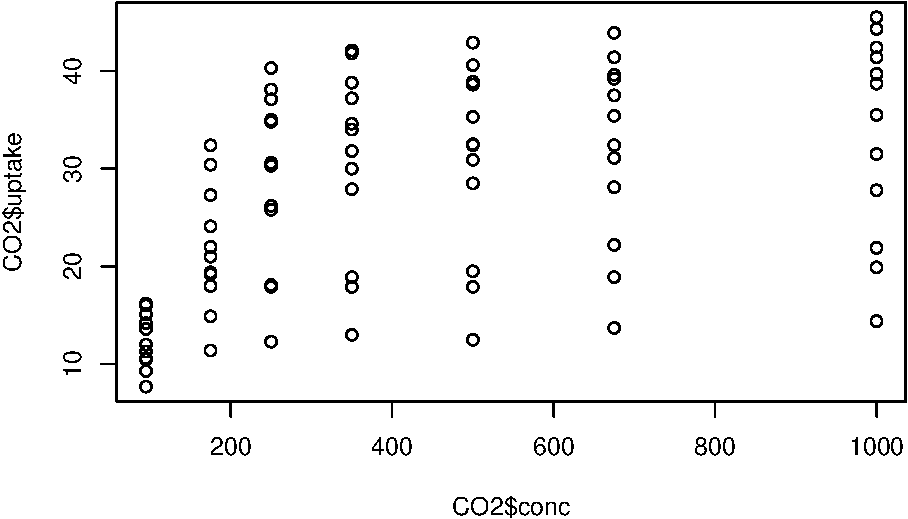
\includegraphics{Plotting_JB_files/figure-latex/unnamed-chunk-13-1.pdf}

Or, you can just use the boxplot() function directly, but use the help
file to understand the different arguments:

\begin{Shaded}
\begin{Highlighting}[]
\NormalTok{?boxplot}
\CommentTok{# Since we want to look at the differences by species, we would use the formula version:}
\KeywordTok{boxplot}\NormalTok{(}\DataTypeTok{formula =}\NormalTok{ Petal.Length }\OperatorTok{~}\StringTok{ }\NormalTok{Species, }\DataTypeTok{data =}\NormalTok{ iris)}
\end{Highlighting}
\end{Shaded}

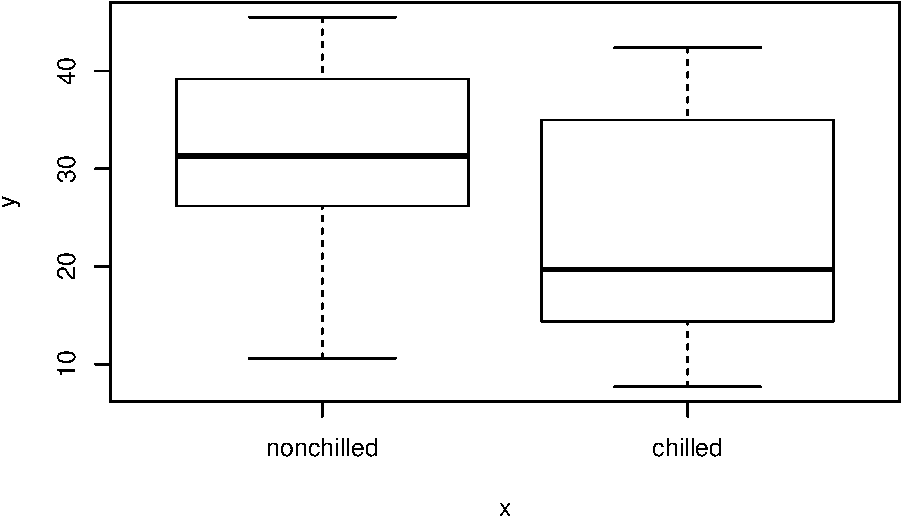
\includegraphics{Plotting_JB_files/figure-latex/unnamed-chunk-14-1.pdf}

\begin{Shaded}
\begin{Highlighting}[]
\CommentTok{# Tip: the tilde signifies that the left side variable is a response (i.e., the "y" variable) to the right side variable (i.e., the "x" variable). The same notation is used in statistical modeling}
\end{Highlighting}
\end{Shaded}

\hypertarget{what-makes-a-good-visualization}{%
\section{What makes a good
visualization?}\label{what-makes-a-good-visualization}}

\hypertarget{plots-should-have-a-purpose-a-clearly-defined-set-of-variables-and-a-message-being-conveyed.}{%
\section{\texorpdfstring{* Plots should have a \textbf{purpose}, a
clearly defined set of variables and a message being
conveyed.}{* Plots should have a purpose, a clearly defined set of variables and a message being conveyed.}}\label{plots-should-have-a-purpose-a-clearly-defined-set-of-variables-and-a-message-being-conveyed.}}

\hypertarget{plots-should-be-succinct-and-uncluttered-so-as-to-allow-easy-interpretation-of-the-purpose.}{%
\section{* Plots should be succinct and uncluttered so as to allow easy
interpretation of the
purpose.}\label{plots-should-be-succinct-and-uncluttered-so-as-to-allow-easy-interpretation-of-the-purpose.}}

\hypertarget{plots-should-be-comprehensive-representing-the-data-accurately-and-fairly.}{%
\section{* Plots should be comprehensive, representing the data
accurately and
fairly.}\label{plots-should-be-comprehensive-representing-the-data-accurately-and-fairly.}}

\hypertarget{explore-the-data-with-simpler-plots-then-make-them-pretty}{%
\section{Explore the data with simpler plots, then make them
pretty!}\label{explore-the-data-with-simpler-plots-then-make-them-pretty}}

\hypertarget{scatterplots}{%
\section{Scatterplots
------------------------------------------------------------------------------------------------}\label{scatterplots}}

\hypertarget{changing-ambient-co2-should-affect-co2-uptake---less-co2-available-might-imply-a-slower-uptake-rate.-can-we-visualize-this}{%
\section{Changing ambient CO2 should affect CO2 uptake - less CO2
available might imply a slower uptake rate. Can we visualize
this?}\label{changing-ambient-co2-should-affect-co2-uptake---less-co2-available-might-imply-a-slower-uptake-rate.-can-we-visualize-this}}

\hypertarget{we-have-two-numeric-vectors-within-the-dataframe-this-is-a-good-candidate-for-a-simple-scatterplot}{%
\section{We have two numeric vectors within the dataframe ; this is a
good candidate for a simple
scatterplot}\label{we-have-two-numeric-vectors-within-the-dataframe-this-is-a-good-candidate-for-a-simple-scatterplot}}

\begin{Shaded}
\begin{Highlighting}[]
\KeywordTok{class}\NormalTok{(CO2}\OperatorTok{$}\NormalTok{conc)}
\end{Highlighting}
\end{Shaded}

\begin{verbatim}
## [1] "numeric"
\end{verbatim}

\begin{Shaded}
\begin{Highlighting}[]
\KeywordTok{class}\NormalTok{(CO2}\OperatorTok{$}\NormalTok{uptake)}
\end{Highlighting}
\end{Shaded}

\begin{verbatim}
## [1] "numeric"
\end{verbatim}

\hypertarget{plot-opens-up-the-plotting-window-defaulting-to-the-ranges-of-the-data-initially-passed-to-plot}{%
\section{Plot opens up the plotting window defaulting to the ranges of
the data initially passed to
plot()}\label{plot-opens-up-the-plotting-window-defaulting-to-the-ranges-of-the-data-initially-passed-to-plot}}

\begin{Shaded}
\begin{Highlighting}[]
\KeywordTok{plot}\NormalTok{(}\DataTypeTok{x =}\NormalTok{ CO2}\OperatorTok{$}\NormalTok{conc, }\DataTypeTok{y =}\NormalTok{ CO2}\OperatorTok{$}\NormalTok{uptake)}
\end{Highlighting}
\end{Shaded}

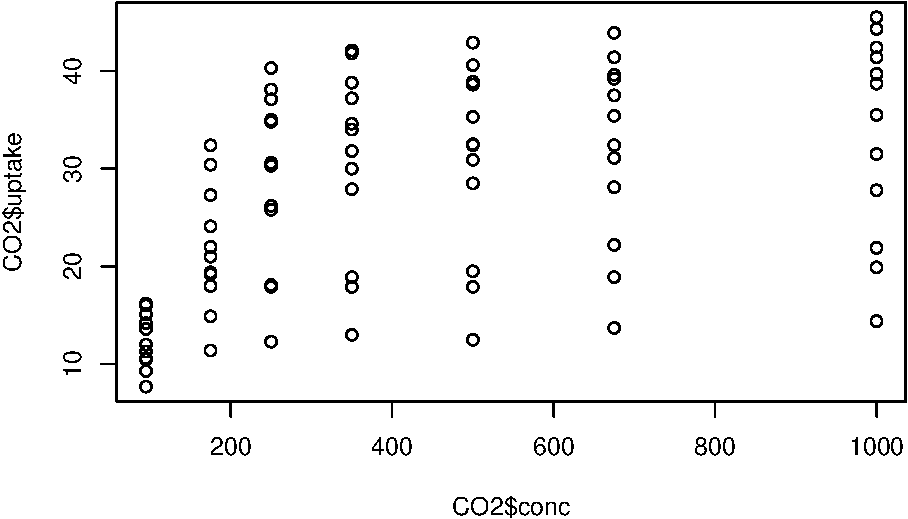
\includegraphics{Plotting_JB_files/figure-latex/unnamed-chunk-16-1.pdf}
\# Commentary: There's some increase in uptake as the concentration
gradient increases, but it doesn't really increase much after
\textasciitilde{}250 uL/L. It may imply that CO2 concentration is only a
limiting factor at very low levels and does not drive uptake at higher
concentrations

\hypertarget{lets-format-the-plot-a-little-better.}{%
\section{Let's format the plot a little
better.}\label{lets-format-the-plot-a-little-better.}}

\begin{Shaded}
\begin{Highlighting}[]
\KeywordTok{plot}\NormalTok{(}\DataTypeTok{x =}\NormalTok{ CO2}\OperatorTok{$}\NormalTok{conc, }\DataTypeTok{y =}\NormalTok{ CO2}\OperatorTok{$}\NormalTok{uptake, }
     \DataTypeTok{xlab =} \StringTok{'CO2 Concentration uL/L'}\NormalTok{, }
     \DataTypeTok{ylab =} \StringTok{'CO2 Uptake (umol/m^2 sec)'}\NormalTok{, }
     \DataTypeTok{main =} \StringTok{'CO2 Uptake Under Ambient CO2 Concentration Gradient'}\NormalTok{)}
\end{Highlighting}
\end{Shaded}

\includegraphics{Plotting_JB_files/figure-latex/unnamed-chunk-17-1.pdf}

\hypertarget{and-tweak-some-specifications-even-more}{%
\section{And tweak some specifications even
more:}\label{and-tweak-some-specifications-even-more}}

\hypertarget{note-par-is-useful-if-you-want-to-set-plot-specifications-for-the-plotting-window-as-well-as-any-plots-following-but-many-of-the-arguments-could-be-used-directly-in-the-plot-function-too-for-the-specific-plot-e.g.-pch-col-cex.xxx.}{%
\subsection{Note, par() is useful if you want to set plot specifications
for the plotting window, as well as any plots following, but many of the
arguments could be used directly in the plot function too for the
specific plot (e.g., pch, col,
cex.XXX).}\label{note-par-is-useful-if-you-want-to-set-plot-specifications-for-the-plotting-window-as-well-as-any-plots-following-but-many-of-the-arguments-could-be-used-directly-in-the-plot-function-too-for-the-specific-plot-e.g.-pch-col-cex.xxx.}}

\begin{Shaded}
\begin{Highlighting}[]
\NormalTok{?par}
\KeywordTok{par}\NormalTok{(}\DataTypeTok{mar =} \KeywordTok{c}\NormalTok{(}\DecValTok{5}\NormalTok{, }\DecValTok{4}\NormalTok{, }\DecValTok{4}\NormalTok{, }\DecValTok{2}\NormalTok{) }\OperatorTok{+}\StringTok{ }\DecValTok{1}\NormalTok{, }
    \DataTypeTok{cex.lab =} \FloatTok{1.5}\NormalTok{, }
    \DataTypeTok{cex.main =} \DecValTok{2}\NormalTok{, }
    \DataTypeTok{pch =} \DecValTok{19}\NormalTok{)}
\KeywordTok{plot}\NormalTok{(}\DataTypeTok{x =}\NormalTok{ CO2}\OperatorTok{$}\NormalTok{conc, }\DataTypeTok{y =}\NormalTok{ CO2}\OperatorTok{$}\NormalTok{uptake, }
     \DataTypeTok{xlab =} \KeywordTok{expression}\NormalTok{(}\KeywordTok{paste}\NormalTok{(CO[}\DecValTok{2}\NormalTok{] ,}\StringTok{" concentration uL/L"}\NormalTok{)), }
     \DataTypeTok{ylab =} \KeywordTok{expression}\NormalTok{(}\KeywordTok{paste}\NormalTok{(CO[}\DecValTok{2}\NormalTok{], }\StringTok{" uptake umol/"}\NormalTok{, m}\OperatorTok{^}\DecValTok{2}\NormalTok{ ,}\StringTok{"sec"}\NormalTok{)), }
     \DataTypeTok{main =} \KeywordTok{expression}\NormalTok{(}\KeywordTok{paste}\NormalTok{(CO[}\DecValTok{2}\NormalTok{], }\StringTok{" uptake Under Ambient CO2 Concentration Gradient"}\NormalTok{)))}
\end{Highlighting}
\end{Shaded}

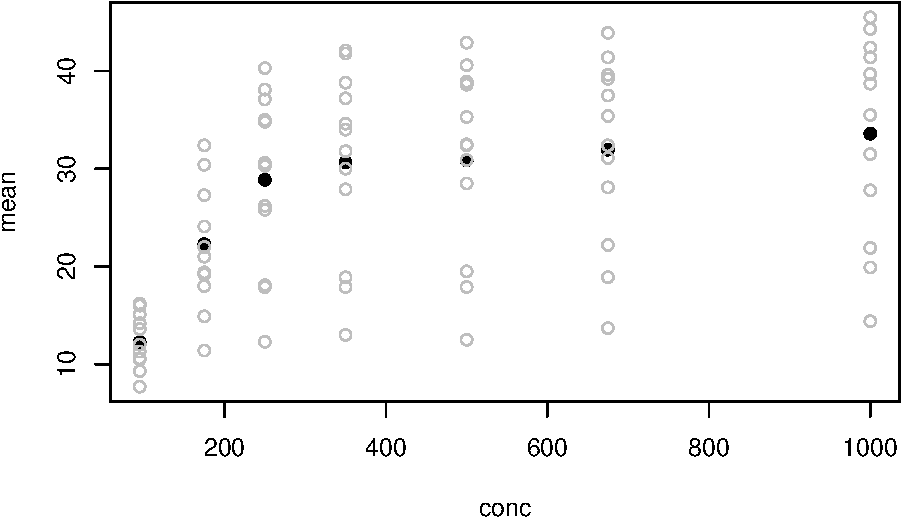
\includegraphics{Plotting_JB_files/figure-latex/unnamed-chunk-18-1.pdf}

\begin{Shaded}
\begin{Highlighting}[]
\KeywordTok{pdf}\NormalTok{(}\StringTok{"co2up.pdf"}\NormalTok{)}
\KeywordTok{par}\NormalTok{(}\DataTypeTok{mar =} \KeywordTok{c}\NormalTok{(}\DecValTok{10}\NormalTok{, }\DecValTok{5}\NormalTok{, }\DecValTok{4}\NormalTok{, }\DecValTok{4}\NormalTok{) , }
    \DataTypeTok{pch =} \DecValTok{19}\NormalTok{,}
    \DataTypeTok{xpd =} \OtherTok{TRUE}\NormalTok{)}

\KeywordTok{palette}\NormalTok{(}\KeywordTok{c}\NormalTok{(}\StringTok{"red"}\NormalTok{, }\StringTok{"blue"}\NormalTok{))}
\KeywordTok{plot}\NormalTok{(}\DataTypeTok{x =}\NormalTok{ CO2}\OperatorTok{$}\NormalTok{conc, }\DataTypeTok{y =}\NormalTok{ CO2}\OperatorTok{$}\NormalTok{uptake, }
     \DataTypeTok{ylim =} \KeywordTok{c}\NormalTok{(}\DecValTok{0}\NormalTok{, }\DecValTok{50}\NormalTok{),}
     \DataTypeTok{xlab =} \KeywordTok{expression}\NormalTok{(}\KeywordTok{paste}\NormalTok{(CO[}\DecValTok{2}\NormalTok{] ,}\StringTok{" concentration uL/L"}\NormalTok{)), }
     \DataTypeTok{ylab =} \KeywordTok{expression}\NormalTok{(}\KeywordTok{paste}\NormalTok{(CO[}\DecValTok{2}\NormalTok{], }\StringTok{" uptake umol/"}\NormalTok{, m}\OperatorTok{^}\DecValTok{2}\NormalTok{ ,}\StringTok{"sec"}\NormalTok{)), }
     \DataTypeTok{main =} \KeywordTok{expression}\NormalTok{(}\KeywordTok{paste}\NormalTok{(CO[}\DecValTok{2}\NormalTok{], }\StringTok{" uptake Under Ambient CO2 Concentration Gradient"}\NormalTok{)), }
     \DataTypeTok{col =}\NormalTok{ CO2}\OperatorTok{$}\NormalTok{Treatment)}
\KeywordTok{legend}\NormalTok{(}\DataTypeTok{x =} \DecValTok{300}\NormalTok{,}
       \DataTypeTok{y =} \DecValTok{-15}\NormalTok{,}
       \DataTypeTok{legend =} \KeywordTok{levels}\NormalTok{(CO2}\OperatorTok{$}\NormalTok{Treatment),}
       \DataTypeTok{col =} \DecValTok{1}\OperatorTok{:}\DecValTok{2}\NormalTok{,}
       \DataTypeTok{pch =} \DecValTok{19}\NormalTok{,}
       \DataTypeTok{bty =} \StringTok{"n"}\NormalTok{,}
       \DataTypeTok{horiz =}\NormalTok{ T)}

\KeywordTok{palette}\NormalTok{(}\KeywordTok{c}\NormalTok{(}\StringTok{"green"}\NormalTok{, }\StringTok{"grey"}\NormalTok{))}
\KeywordTok{plot}\NormalTok{(}\DataTypeTok{x =}\NormalTok{ CO2}\OperatorTok{$}\NormalTok{conc, }\DataTypeTok{y =}\NormalTok{ CO2}\OperatorTok{$}\NormalTok{uptake, }
     \DataTypeTok{ylim =} \KeywordTok{c}\NormalTok{(}\DecValTok{0}\NormalTok{, }\DecValTok{50}\NormalTok{),}
     \DataTypeTok{xlab =} \KeywordTok{expression}\NormalTok{(}\KeywordTok{paste}\NormalTok{(CO[}\DecValTok{2}\NormalTok{] ,}\StringTok{" concentration uL/L"}\NormalTok{)), }
     \DataTypeTok{ylab =} \KeywordTok{expression}\NormalTok{(}\KeywordTok{paste}\NormalTok{(CO[}\DecValTok{2}\NormalTok{], }\StringTok{" uptake umol/"}\NormalTok{, m}\OperatorTok{^}\DecValTok{2}\NormalTok{ ,}\StringTok{"sec"}\NormalTok{)), }
     \DataTypeTok{main =} \KeywordTok{expression}\NormalTok{(}\KeywordTok{paste}\NormalTok{(CO[}\DecValTok{2}\NormalTok{], }\StringTok{" uptake Under Ambient CO2 Concentration Gradient"}\NormalTok{)), }
     \DataTypeTok{col =}\NormalTok{ CO2}\OperatorTok{$}\NormalTok{Type)}
\KeywordTok{legend}\NormalTok{(}\DataTypeTok{x =} \DecValTok{300}\NormalTok{,}
       \DataTypeTok{y =} \DecValTok{-15}\NormalTok{,}
       \DataTypeTok{legend =} \KeywordTok{levels}\NormalTok{(CO2}\OperatorTok{$}\NormalTok{Type),}
       \DataTypeTok{col =} \DecValTok{1}\OperatorTok{:}\DecValTok{2}\NormalTok{,}
       \DataTypeTok{pch =} \DecValTok{19}\NormalTok{,}
       \DataTypeTok{bty =} \StringTok{"n"}\NormalTok{,}
       \DataTypeTok{horiz =}\NormalTok{ T)}

\KeywordTok{dev.off}\NormalTok{()}
\end{Highlighting}
\end{Shaded}

\begin{verbatim}
## pdf 
##   2
\end{verbatim}


\end{document}
